\documentclass{article}

\usepackage[hidelinks]{hyperref}
\usepackage[T1]{fontenc}
\usepackage{amsmath}
\usepackage{amssymb}
\usepackage{amsthm}
\usepackage{listings}
\usepackage[dvipsnames]{xcolor}
\usepackage{graphicx}
\graphicspath{ {./img/} }
\usepackage{subfig}
\usepackage{comment}



\usepackage[justification=centering]{caption}
\usepackage{geometry} % geometry package for mentioning margin length
\geometry{
 a4paper,
 total={170mm,257mm},
 left=30mm,
 right=30mm,
 top=30mm,
 bottom=30mm
 }
\usepackage{listings}
\usepackage{bm}

\author{D'Urso Mattia}
\date{\today}
\title{\small Computer Vision project \\ \LARGE Learning the Super Resolution Space}

%\hypersetup{colorlinks}
\begin{document}
\maketitle
\clearpage
\tableofcontents
\clearpage

\section{Introduction}
% Area
%compuer vision dal 19mai % TO CHECK
Within the Computer Science area, one of the topics of high interest has always been Artificial Intelligence (AI). We define AI as the simulation of human intelligence computed by machines. Specific applications of AI include natural language processing, speech recognition, and computer vision (CV). The latter is one of the most-studied topics, we can define it as a subset of AI that deals in teaching machines how to understand images.
% approcci negli anni image processing -> deep learning
% traditional > on small daatsets, full trasparent

% Problem
%diversi problemi (lista) tra cui super Resolution % attuale: cit cose super res NVDIA DLSS
The first problem CV tried to solve was to make a robot "see" the world by connecting a video camera to a computer, around the 1960s at MIT. Today the field made several steps further, and there are many more problems that the CV aims to solve. Among these, we find image classification, the task of deciding whether class images belong, object detection, which is finding and classifying objects within an image, and semantic segmentation, which consists of grouping the parts of an image that belong to the same class of objects. With the advancement of technology, new challenges presented themselves, like the problem of the upscaling image. It is about reconstructing a meaningful high-resolution image (HR) from a low-resolution image (LR). This task is called Image Super-Resolution (SR). SR is a fundamentally ill-posed problem. In fact, for a given LR image, there exist infinitely many compatible HR predictions. Nevertheless, SR has several real-world applications such as surveillance (e.g., face recognition in upscaled images) and media sharing (e.g., sending LR images and upscaling on the fly). This issue is of interest also to large companies like NVIDIA that developed the deep learning super sampling (DLSS) \cite{dlss} to use it on its GPUs when rendering video game frames. The aim is to render the game at LR (e.g., 1920$\times$1080) and then use DLSS to upscale images to HR (e.g., 3840$\times$2160). In this way, it is possible to play HR games with less computational rendering power. 

% Goal 
Regarding the SR problem, there are also some public competitions, such as the 2021 ``Learning the Super-Resolution Space'' challenge, held as part of the $6th{th}$ edition of the New Trends in Image Restoration and Enhancement (NTIRE) workshop, in conjunction with the 2021 Conference on Computer Vision and Pattern Recognition (CVPR). The goal of the ``Learning the Super-Resolution Space'' challenge is to develop an SR method that can upscale downscaled images sampled from the space of plausible HR images. More formally, given an HR image $IMG$ sampled from a space of images $S_{IMG}$ and downscaled to an LR image $img$, the aim is to find a method $f$ that

\begin{displaymath}
    IMG' = f(img)
\end{displaymath}

\noindent where $IMG'$ is an HR image and it belongs to a plausible space of images. \\

In section~\ref{sec:sota} we describe the State-of-the-art approaches for the SR task. In section~\ref{sec:model} we describe in detail how the NTIRE flow models for SR work. In section~\ref{sec:eval} we run some tests with the aforementioned flow models. Finally, in section~\ref{sec:conc} se we draw the conclusions.

\subsection{NTIRE challenge details}
The challenge contains two tracks, targeting 4X and 8X super-resolution respectively. The running methods shall achieve the highest possible photo-realism and be consistent with the input LR image. The methods are tested with the following metrics \cite{ntire21}. %(https://openaccess.thecvf.com/content/CVPR2021W/NTIRE/papers/Lugmayr_NTIRE_2021_Learning_the_Super-Resolution_Space_Challenge_CVPRW_2021_paper.pdf) 
\begin{itemize}
    \item[$-$] \textbf{Diversity score}: This metric aims to measure how well the SR image of ground truth is represented in the predicted space. From the predicted image $IMG'$ and the original image $IMG$, $k$ random patches are sampled $y_k \ in \mathbb{R}^{N \times N \times 3}$ and the similarity is calculated with a distance metric $d$.  To obtain the significant diversity that the samples represent, testers calculate by how much the minimum distance from the reference patch decreases when $M$ samples are used,

    \begin{equation}
        S_M = \frac{1}{\overline{d}_M}(\overline{d}_M - \frac{1}{K}\sum^K_{k=1} min\{d(y_k, \hat{y}_k^i)\}^M_{i=1})
    \end{equation}
    where 
    \begin{equation}
        \overline{d}_M = min \{\frac{1}{K}\sum^K_{k=1}d(y_k, \hat{y}_k^i)\}^M_{i=1}
    \end{equation}
    Notice that $S_M \in [0,1]$ where $S_M=0$ means no diversity (deterministic predictions) and $S_M=1$ means
    that the ground-truth HR image was exactly captured by one of the generated samples.

    \item[$-$] \textbf{LR-PSNR}: This metric aims to measure the amount of information retained in the SR image compared to the LR image measuring the LR-PSNR. It is calculated as the PSNR between the input LR image and the predicted sample resized with the given bicubic kernel. The goal of this challenge is to obtain an LR-PSNR of at least 45dB.

    \item[$-$] \textbf{Mean Opinion Rank}: This metric aims to assess the degree of photorealism of an image. This task is performed by humans on three different 80$\times$80 pixels cutouts of the 100 images in the test set. Each task is performed by five different users. Finally, the user is asked to rank the cutouts according to their opinion.
\end{itemize}

\noindent The participating methods are ranked according to each metric. These ranks then are combined into a final score. The first method wins the challenge.

% Task
After AlexNet won the 2012 ImageNet Large Scale Visual Recognition Challenge, deep learning (DL) methods became increasingly popular in the CV field because they performed significantly better than methods used up to that point in a wide set of tasks. Following this trend, during NTIRE 2021 the most common approach was the use of DL methods. In particular, Generative Adversarial Networks (GANs), Variational AutoEncoders (VAEs), GANs trained with implicit maximum likelihood estimation (IMLE), and Flow models were used. \\ %In this report we discuss the last method. \\



\newpage
\section{State-of-the-art architectures for Super Resolution}\label{sec:sota}
In this section we describe the idea of the approaches used during the 2021 ``Learning the Super-Resolution Space'' challenge. They are four approaches based on DL techniques.


\subsection{Generative Adversarial Networks}
The Generative Adversarial Networks was introduced in \cite{gans} in 2014. Goodfellow's team proposed two networks that act as generator and discriminator. The former network aims to generate data from random noise, while the second method must decide whether the data generated is realistic or not. The two models are trained alternately, so when the generator is trained, the discriminator is kept constant and vice versa. Figure~\ref{img:gan} show the base GAN architecture.
\begin{figure}[h]
    \centering
    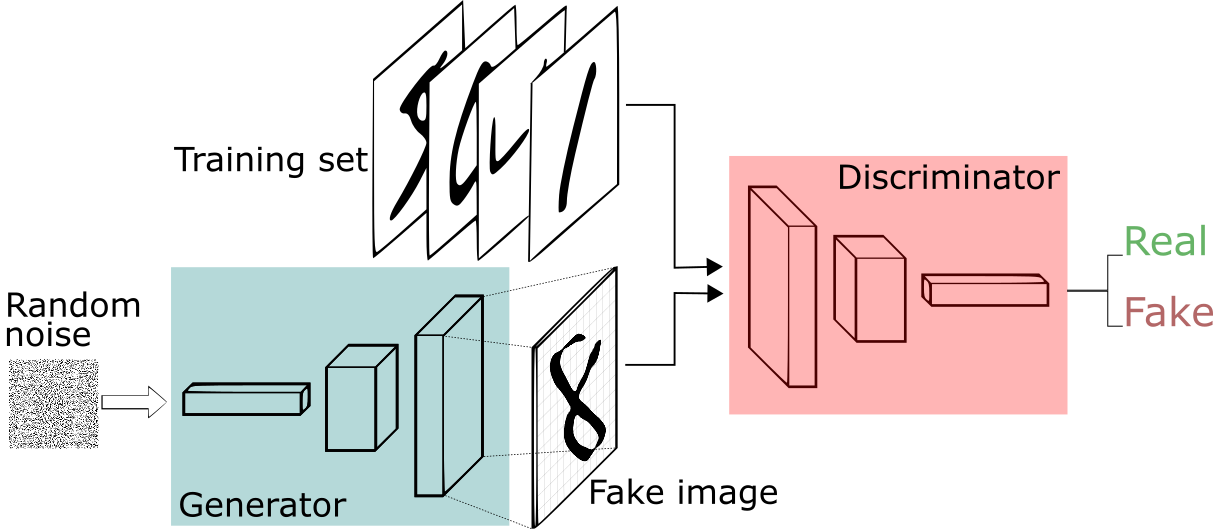
\includegraphics[scale=.3]{gan.png}
    \caption{Generative Adversarial Networks architecture applied to images.}
    \label{img:gan}
\end{figure}

Since the GAN approach is deterministic and has usually a low LR-PSNR, few teams add some layers to make it stochastic and LR consistent. The former layers add some random noise during the inference time, while the latter layers are based on \cite{esp} that is a GUI based method to interactively exploring the manifold of possible HR images. 

\subsection{Variational Auto-Encoders}
The Variational Auto-Encoder (VAE) architecture was introduced in \cite{vae}. VAE is an autoencoder that, unlike AutoEncoders, encodes data in two vectors that are means ($\mu$) and standard deviations ($\sigma$). During the training, those vectors are constrained to ensure that the latent distribution they describe has some properties. To achive stochastic image generation some noise is add to the discriminator's input.

\begin{figure}[h]
    \centering
    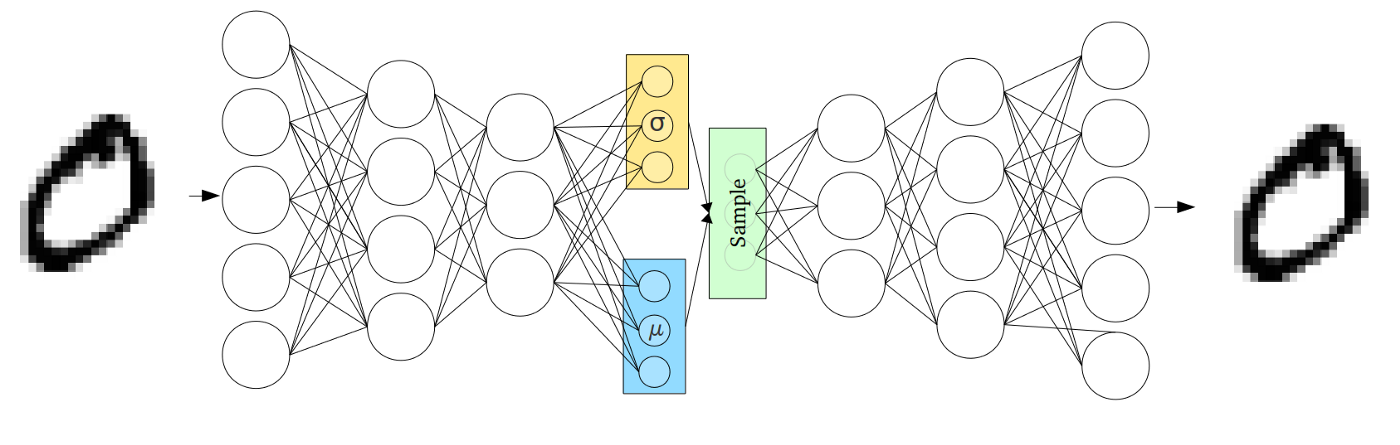
\includegraphics[scale=.3]{vae.png}
    \caption{Variational Auto-Encoders architecture applied to an image.}
    \label{img:vae}
\end{figure}


%used for data reduction and generation
%https://towardsdatascience.com/understanding-variational-autoencoders-vaes-f70510919f73

\subsection{Implicit Maximum Likelihood Estimator}
Implicit Maximum Likelihood Estimator (IMLE) is a technique to train implicit models (e.g., GANs) introduced in \cite{imle}. Assuming that we do not know the distribution of the model and have only a finite set of i.i.d. samples, more samples are expected to be found near the data examples than elsewhere. Therefore, the aim is to minimize the distance from each data example to the nearest sample. The IMLE is defined as
\begin{equation}
    \hat{\theta}_{IMLE} = \normalfont{arg} \min_{\theta} \mathbb{E}_{\tilde{x}_1^{\theta}, ..., \tilde{x}_m^{\theta}} \biggl[ \sum^n _{i=1} \min_{j \in [m]} ||\tilde{x}_j^{\theta}-x_i||_2^2\biggr]
\end{equation}
where $x_1, ... x_n$ is the set of $n$ samples and $P_\theta$ is some unknown parameterized probability with density $p_\theta$. $\tilde{x}_1^\theta, ... \tilde{x}^\theta_m$ is the set of i.i.d. samples from $P_\theta$ with $m \geq n$.
\colorbox{red}{ADD: https://arxiv.org/pdf/1610.03483.pdf}

\subsection{Flow models}
Flow models are particular architectures in which data (usually images) flows in both directions. They aim to learn the distribution of HR data $p_{y|x}(y|x, \theta)$ (where $x$ is the encoded nHR sample, $y$ is the HR sample and $\theta$ are the parameters of the function $f$), and not only an injective correspondence $x \rightarrow y$. In this way, the model can sample multiple HR samples from the learned plausible distribution given one LR sample. The model is also required to be invertible w.r.t $y$, which means given the latent encoding $z = f_{\theta}(y;x)$ we can reconstruct $y$ as $y = f_{\theta}^{-1}(z;x)$. As in the previous models, also flow models accept noise to generate stochastic images.
\begin{figure}[h]
    \centering
    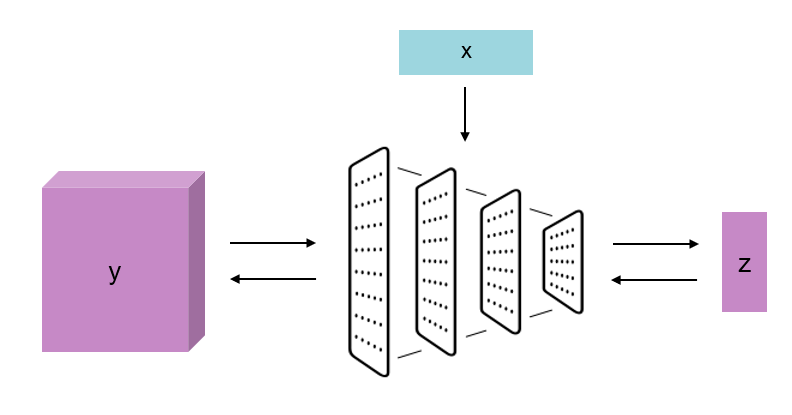
\includegraphics[scale=.6]{flow.png}
    \caption{Normalizing flow model architecture. y is the HR image, x is the encoded HR image and z is the latent vector.}
    \label{img:vae}
\end{figure}


\newpage
\section{Flow models for Super Resolution}\label{sec:model} %https://lilianweng.github.io/posts/2018-10-13-flow-models/
In this sction we describe in detail \cite{srFlow} and the two variations \cite{srFlow-da,ncsr} that compete in the challenge. Some details are in common like the loss function used and the majority of the layers.
%Early DL approaches to the SR task trained feed-forward architectures using $L_1$\footnote{$L_1(y,\hat{y}) = \sum^n_{i=1} |y-\hat{y}|$} or $L_2$\footnote{$L_2(y,\hat{y}) = \sum^n_{i=1} (y-\hat{y})^2$} losses. The problem with these methods is they reduce high frequencies resulting in blurred images because of the average nature of the aforementioned loss functions. To address this problem more recent approaches introduced adversarial training and perceptual losses functions (work by summing all the squared errors between all the pixels and computing the mean). Adversarial methods obtain better results while they can compute a single prediction for an image. They also use multiple loss functions during the training phase with careful parameter tuning.

\subsection{Flow models' loss function}
Flow models are trained with a single loss function that is negative log-likelihood\footnote{$\mathcal{L}(\theta; x, y) = - \text{log}\:p_{y|x}(y|x, \theta)$} (NLL), which simplifies training. The core idea of normalizing flow is to parametrize the distribution $p_{y|x}$ using a neural network $f_\theta$.  The distribution $p_{y|x}$ can be computed as
\begin{equation}
    \label{eq:probyx}
    p_{y|x}(y|x,\theta) = p_z (f_{\theta}(y;x))  \bigg | det \frac{\partial f_{\theta}}{\partial y}(y;x) \bigg |
\end{equation}
which is derived by applying the change-of-variables formula for densities, where the second factor is the resulting volume scaling given by the absolute value of the determinant of the Jacobian $\frac{\partial f_{\theta}}{\partial y}$. Equation~\ref{eq:probyx} allows us to train the network by minimizing the negative log-likelihood for training samples pairs $(x, y)$ as follows.

\begin{equation}
    \label{eq:nprobyx}
    \mathcal{L}(\theta; x,y) = -\textnormal{log} \: p_{y|x}(y|x,\theta) = -\textnormal{log} \: p_z (f_{\theta}(y;x))  -\textnormal{log} \: \bigg | det \frac{\partial f_{\theta}}{\partial y}(y;x) \bigg |
\end{equation}
In order to achieve a tractable expression of the second term in equation~\ref{eq:nprobyx}, the neural network $f_\theta$ is decomposed into a sequence of $N$ invertible layers $h^{n+1}= f^n_\theta(h^n, g_\theta(x))$, where $h^0 = y$ and $h^N = z$. We let the LR image to first be encoded by a shared deep CNN $g_{\theta}(x)$ that extracts a rich representation suitable for conditioning in all flow-layers. By applying the chain rule along with the multiplicative property of the determinant \cite{dens}, the NLL objective in equation~\ref{eq:probyx} can be expressed as

\begin{equation}
    \label{eq:fnprobyx}
    \mathcal{L}(\theta; x,y) = -\textnormal{log} \: p_{z}(z) = -\sum^{N-1}_{n=0}   -\textnormal{log} \: \bigg | det \frac{\partial f_{\theta}^n}{\partial h^n}(h^n;g_\theta(x)) \bigg |
\end{equation}

\noindent The following flow models use equation~\ref{eq:fnprobyx} for the training.


\subsection{SRFlow: Learning the Super-Resolution Space with Normalizing Flow}
The Super-Resolution using Normalizing Flow model (SRFlow) \cite{srFlow} consists of the invertible flow network $f_{\theta}$ and the LR encoder $g_{\theta}$. The flow network is organized into $L$ levels, each operating at a resolution of $\frac{H}{2^l}\times\frac{W}{2^l}$, where $l \in \{1, ..., L\}$ is the level number and $H\times W$ is the HR resolution (e.g., let an input image be $3\times 512 \times 512$, at level 2 will be $48 \times 128 \times 128$, at level 4 will be $768 \times 32 \times 32$, and so on.). Each level itself contains $K$ number of flow steps. To achieve tractable expressions the neural network $f_\theta$ is decomposed into a sequence of $N$ layers $h^{n+1} = f_\theta ^n (h^n; g_\theta(x))$, where $h^0 = y$ and $h^N = z$. These layers can be easly inverted and derived.
%describing the loss ?

The LR encoder $g_{\theta}$ is a Residual-in-Residual Dense Blocks (RRDB) \cite{rrdb} without any batch normalization layers and the final upscaling layers. To capture a richer representation of the LR image at multiple levels, the researchers additionally concatenate the activations after each RRDB block to form the final output of $g_\theta$.

$f_\theta$ is organized as follows.
\begin{itemize}
    \item The \textbf{squeeze} layer: this layer provides an invertible means to halving the resolution by reshaping each spatial $2 \times 2$ neighborhood into the channel dimension (e.g., $3\times 64 \times 64$ into $12 \times 32 \times 32$). This operation is done to capture correlations and structures over larger distances. Figure~\ref{img:squeeze} graphically shows the operation.
    
    \begin{figure}[h]
        \centering
        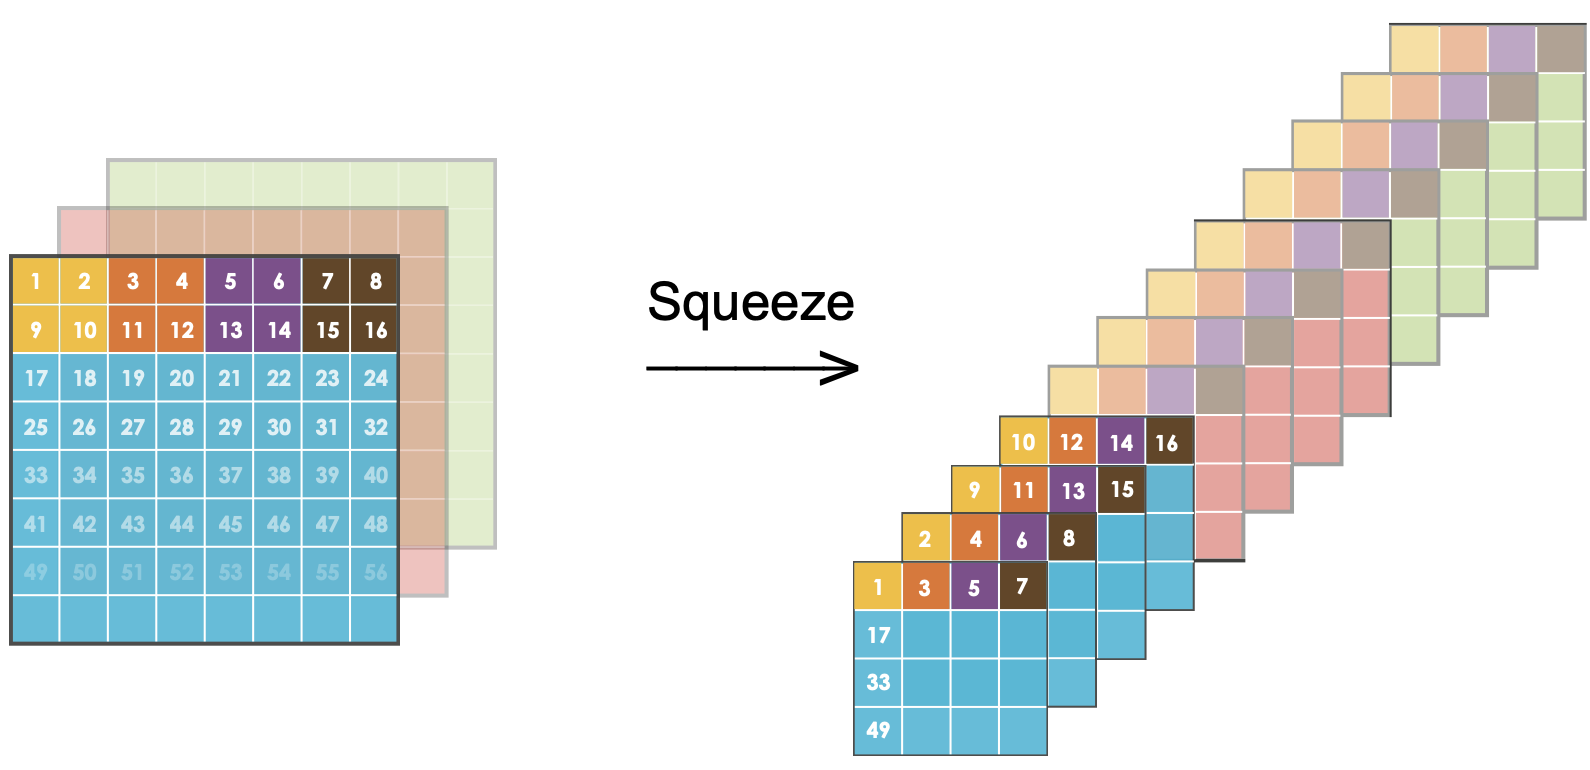
\includegraphics[scale=.3]{squeeze}
        \caption{Visualization of the Squeeze operation.}
        \label{img:squeeze}
    \end{figure}

    \item The \textbf{Transition Step}: this block normalizes and permutes the input according to a learned method.
        \begin{itemize}
            \item \textbf{Actnorm}: This provides a channel-wise normalization through a learned scaling and bias. This layer is ketp in its standard un-conditional form \cite{1x1}.

            \item Invertible $\boldsymbol{1 \times 1}$ \textbf{Convolution}:  this layer is a $1 \times 1$ convolution with equal number of input and output channels, which is a generalization of a permutation operation \cite{1x1}. According to \cite{order}, the ordering of the dimensions can be critical to the training of the model.
        \end{itemize}

    \item The \textbf{Conditional Flow Step}: this block passes the input in another Actnorm layer and $1 \times 1$ convolutional layer. Then, add the conditional information in two steps.
        \begin{itemize}
            \item \textbf{Affine Injector}: this layer directly affects all channels and spatial locations in the activation map $h^n$. This is achieved by predicting an element-wise scaling and bias using only the conditional encoding $u = g_{\theta}(x)$,
            \begin{equation}
                h^{n+1} = \text{exp}\:(f_{\theta, s}(u)) \cdot h^n + f_{\theta, b}(u)
            \end{equation}
            where $f_{\theta, s}$ and $f_{\theta, b}$ can be any network, SRFlow uses a block that consists of $3 \times 3$ convolution, actnorm, ReLU, $1 \times 1$ convolution, actnorm, ReLU, and $3 \times 3$ conv. The exp power is used to have positive values in easy differentible way.

            \item \textbf{Conditional Affine Coupling}: this layer allows applying complex unconstrained conditional learned functions that act on the normalizing flow, without harming its invertibility. The layer splits on half the input $\text{split}(h^{n})= h^{n}_A, h^{n}_B$ along the channel dimension. Then the following transformation on the bypassed half $h^n_A$ and conditional features $u$ is computed
            \begin{equation}
                h^{n+1} = \begin{cases}
                    h^{n+1}_A = h^{n}_A, \:
                    h^{n+1}_B = \text{exp}\:(f_{\theta, s}( h^{n+1}_A; u)) \cdot h^n_B + f_{\theta, b}( h^{n+1}_A; u)
                \end{cases}
            \end{equation}  
            The network architectures of $f_{\theta, s}$ and $f_{\theta, b}$ are similar to those of the Affine Injector, described above. The only difference is that $u$ is resized to the resolution of $h^{n}_A$, then it is concatenated to $h^{n+1}_A$ along the channel dimension. Note that $h^{n+1}$ is a couple.
        \end{itemize}
    \item \textbf{Split} layer: this layer splits the given input in two halfs along the channel dimension. % But why
    \end{itemize}
\noindent Figure~\ref{img:model} graphically shows a representation of the model.

\begin{figure}[h]
    \centering
    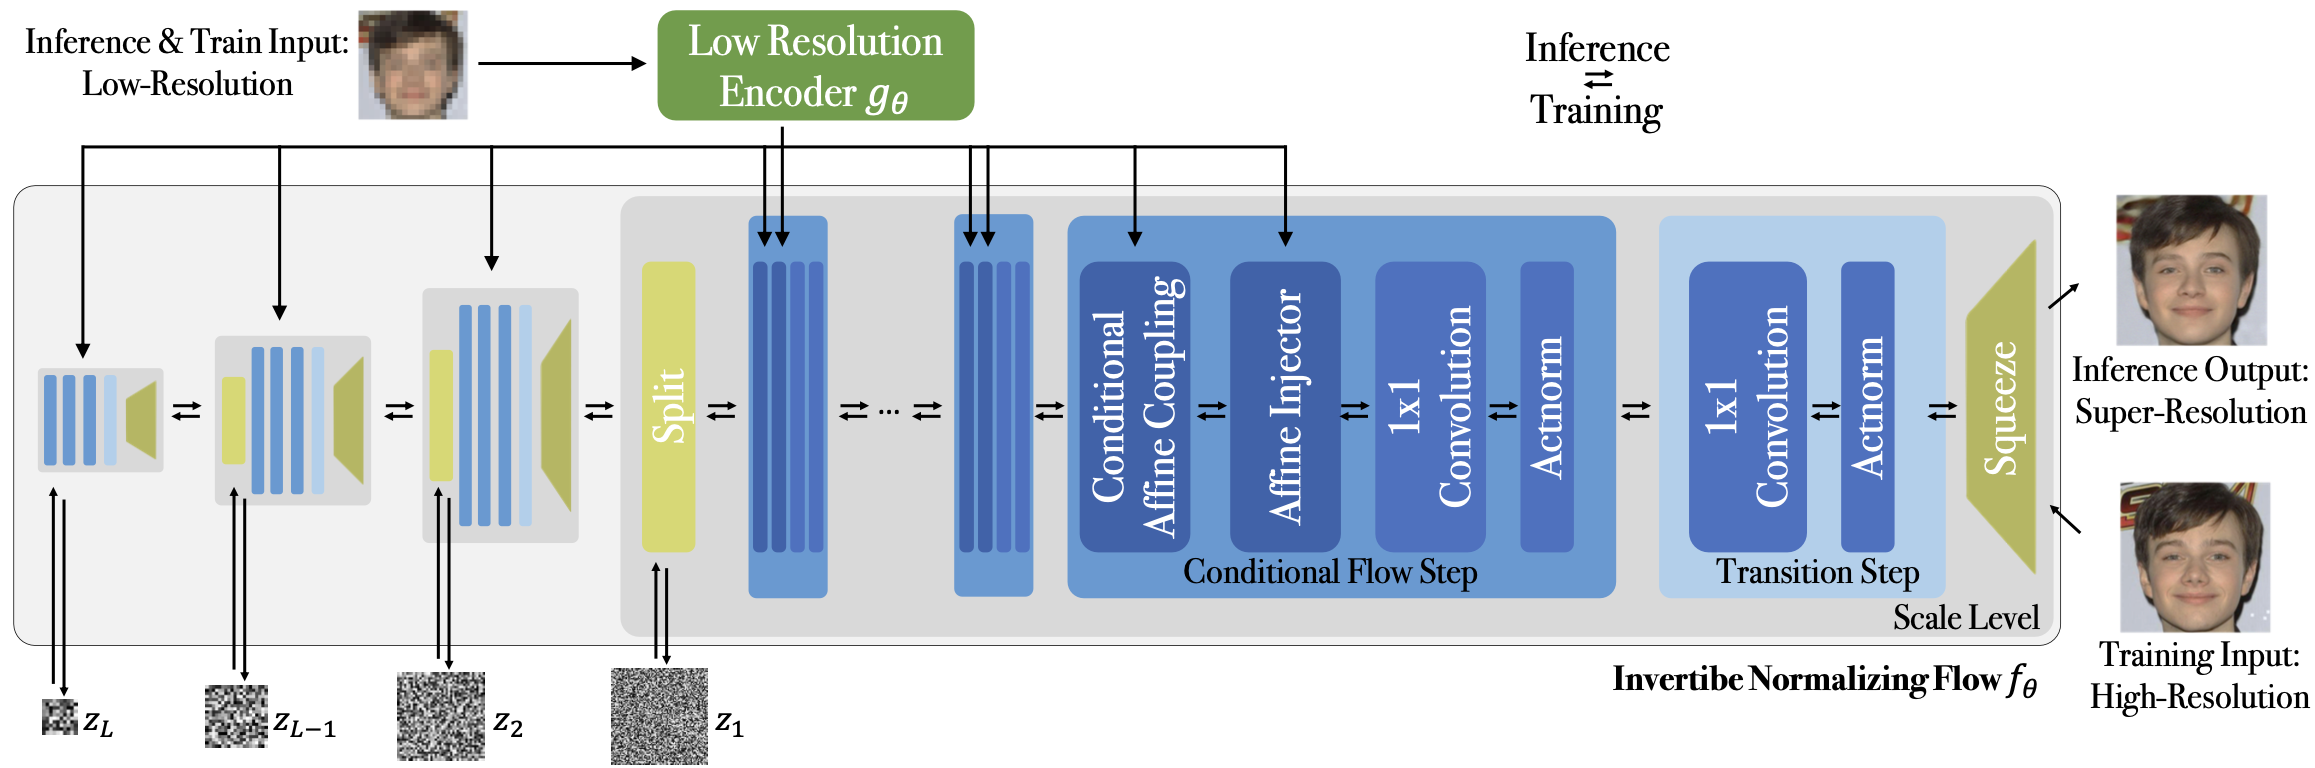
\includegraphics[scale=.38]{model}
    \caption{Super-Resolution using Normalizing Flow's architecture.}
    \label{img:model}
\end{figure}



\subsection{SRFlow-DA: Super-Resolution using Normalizing Flow with Deep Convolutional Block}
Super-Resolution using Normalizing Flow with Deep convolutional block in the Affine couplings (SRFlow-DA) \cite{srFlow-da} model is an architecture based on SRFlow that increases the SR quality while reducing the model size and the training time. The idea is to improve the perfomance enlarging receptive field\footnote{A Receptive Field (RF) is defined as the size of the region in the input that produces the output feature. \cite{rec} shows applying a stack of smaller filters is equivalent and more efficent than a bigger one} size in the single flow step. The SRFlow model has an equivalent RF of $5 \times 5$ while the SRFlow-DA model has a RF of $13 \times 13$, plus the number of flow steps has been reduced from 16 to 6. These two changes reduced the number of parameters from 22.8M (SRFlow) to 8.7M (SRFlow-DA) improving training and inference time. To achive those results, the researchers stacked $3 \times 3$ convolutional layers followed by ReLU activation except for the last convolutional layer. $s$ and $t$ are emprically estimated coefficents that improves the perfomances. Figure~\ref{fig:dablock} highligths the differences.

    \begin{figure}[h]
        \centering
        \subfloat[Affine coupling in SRFlow.]{{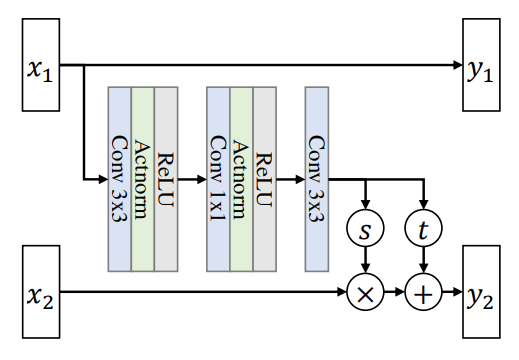
\includegraphics[width=55mm, scale=.4]{dablock_1}}}
        \qquad
        \subfloat[Affine coupling in SRFlow-DA.]{{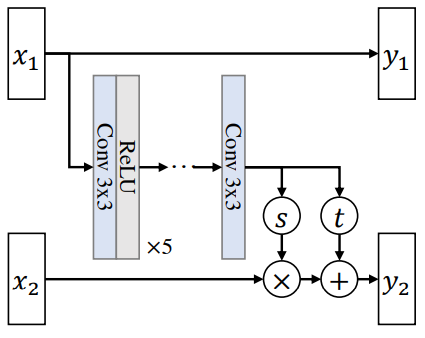
\includegraphics[width=55mm, scale=.25]{dablock_2} }}
        \caption{Comparison between the Affine Coupling layers of the two architectures.}
        \label{fig:dablock}
    \end{figure}


\subsection{Noise Conditional Flow Model for Learning the Super-Resolution Space}
Noise Conditional Flow model for Super-Resolution (NCSR) \cite{ncsr} is an architecture based on SRFlow that improves the diversity of the predicted images by adding noise. In particular, the researchers add noise to the training data and through a new layer called Noise Conditional Layer. NCSR aims to solve also the dimension mismatch problem\footnote{This problem concerns the inability to properly train the model if the size of the data distribution does not match that of the underlying target distribution. \cite{SoftFlow}} typical of Flow models. The architectural difference can be found in the Conditional Flow step. NCSR adds the Noise Conditional Layer in $4^{th}$ position obtaining a block with five elements, as shown in figure~\ref{img:nblock}.

\begin{figure}[h]
    \centering
    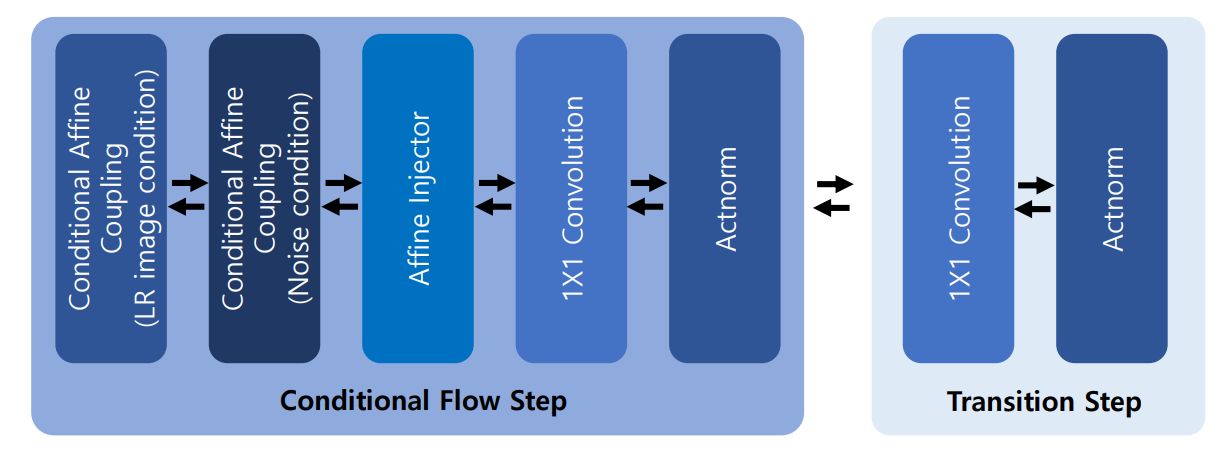
\includegraphics[scale=.35]{nblock}
    \caption{The Conditional Flow block.}
    \label{img:nblock}
\end{figure}

Adding $noise$ to the input data $x$ results in a variation of the distribution of the latent data $z$ during the inference process. To address that the $noise$ used for the input $x$ is resized and added to the LR image $y$ as follows.
\begin{align*}
    x^+ = x + noise \\
    y^+ = y + noise^- \\
    f^{-1}(x^+|y^+) = z 
\end{align*}
where, $x$ is an HR image, $f$ is the invertible model that maps $z$ to $x$ and $y$ is a LR image. 

The second improvement is the introduction of the Noise Conditional Layer, which is a Conditional Affine Coupling layer that uses $noise$ instead of $u$. The idea is to inform noise to the model structure to avoid artifacts caused by the noise injection on $x$. The Noise Affine Conditional layer is designed as follows.
\begin{equation}
    h^{n+1} = \begin{cases}
        h^{n+1}_A = h^{n}_A, \:
        h^{n+1}_B = \text{exp}\:(f_{\theta, s}( h^{n+1}_A; noise)) \cdot h^n_B + f_{\theta, b}( h^{n+1}_A; noise)
    \end{cases}
\end{equation} 

The third contribution is about the dimension mismatch problem. NCSR uses the same approach of \cite{SoftFlow} to overcome it by estimating a perturbed data distribution that is conditioned on noise parameters. The key is to add noise that is obtained from a randomly selected distribution and to use these distribution parameters as conditions. In particular random value $c$ is obtained from uniform distribution $U(0, M)$, where $M$ is 0.1, as \cite{SoftFlow} did. Next, set the to noise distribution $N(0, \Sigma)$, where $\Sigma = c^2I$. Then, noise is sampled from $N(0, \Sigma)$.


Figure~\ref{img:model} graphically shows a representation of the model.

\begin{figure}[h]
    \centering
    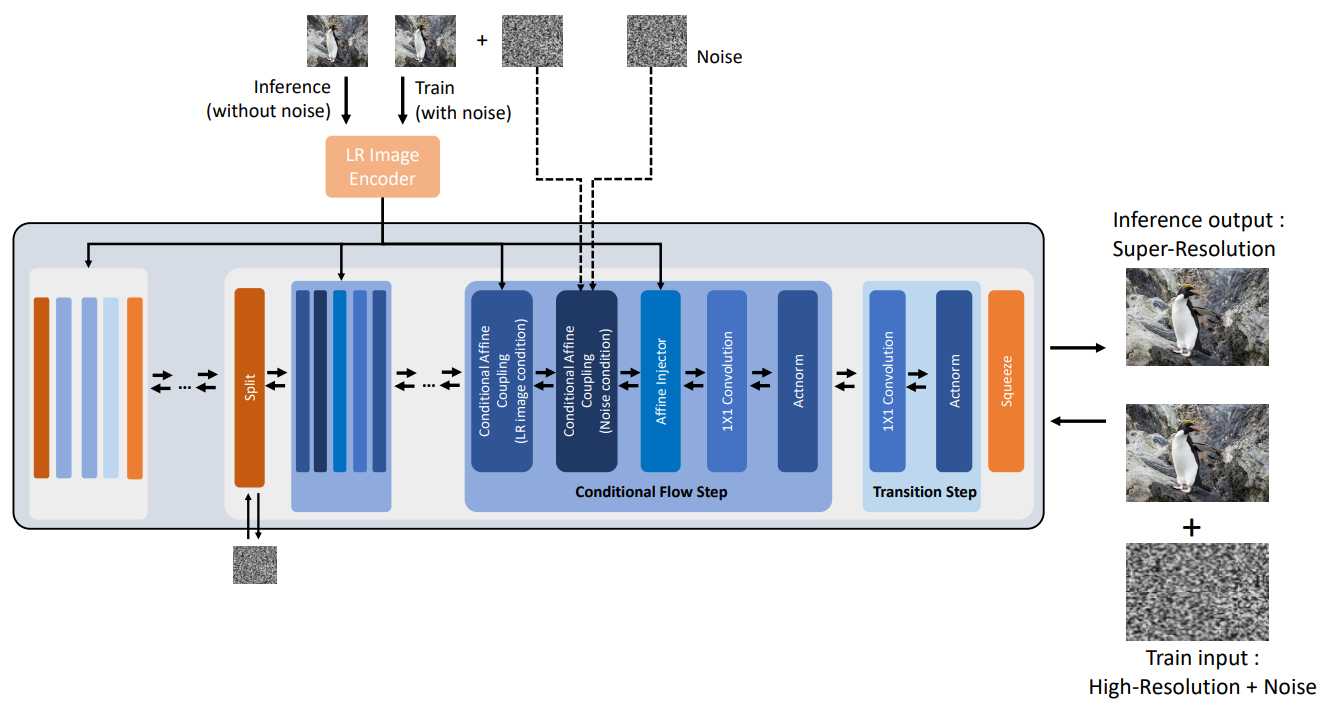
\includegraphics[scale=.45]{model_2}
    \caption{Noise Conditional Flow for Super-Resolution's architecture.}
    \label{img:model_2}
\end{figure}

\begin{comment}
\subsection{Metrics comparison}
The table \ref{tab:4x} and table \ref{tab:8x} show the 4$\times$ and 8$\times$ results of the models on the 100 validation
images of the DIV2K dataset reported in the papers. The arrows near the metric's name indicate the direction for a better result. Best results are highlighted in bold only if the value is reported for all the models. The * means the value is not reported in the original model's paper but in another paper for comparison purposes. Inference time is measured by \cite{srFlow-da} for generating an output image size of 1920$\times$1080. Note that the training times and the inference times are measured on NVIDIA GeForce RTX 2080 TI. 

\begin{table}[h]
    \centering
    \begin{tabular}{ l l l l l l l }
    \hline
    Model & Diversity$\uparrow$ & LPIPS$\downarrow$ & LR-PSNR$\uparrow$ & Params & Train/Infer. time \\
    \hline
    SRFlow      & 25.24* & 0.120 & 50.64 & 22.8M* & 120h*/1.98s*\\
    SRFlow-DA   & 23.55 & 0.121  & \textbf{50.88} & 8.7M  & 33h/1.18s\\
    NCSR        & \textbf{26.72} & \textbf{0.119}  & 50.75 & - & - \\
    \hline
    \end{tabular}
    \caption{4$\times$ results on DIV2K validation set. }
    \label{tab:4x}
\end{table}

\begin{table}[h]
    \centering
    \begin{tabular}{ l l l l l l l }
    \hline
    Model & Diversity$\uparrow$ & LPIPS$\downarrow$ & LR-PSNR$\uparrow$ & Params & Train/Infer. time \\
    \hline
    SRFlow      & 25.28* & 0.272 &  50.09 & 34.1M* & 120h* / 1.97s*\\
    SRFlow-DA   & 23.45 & \textbf{0.261}  & \textbf{50.91} & 13.3M  & 47h / 1.01s\\
    NCSR        & \textbf{26.80} & 0.278  & 44.55 & - & - \\
    \hline
    \end{tabular}
    \caption{8$\times$ results on DIV2K validation set. }
    \label{tab:8x}
\end{table}
\colorbox{red}{ADD COMMENT}
%As we could espect, the SRFlow models has the lowest performances. Looking at the diversity score the NCSR model is the best, this can be explained by the greater amount of noise that is injected in the model. The SRFlow-DA model is the one with largest filters, 
\end{comment}

\newpage
\section{Experiments ?}\label{sec:eval}
%In this section we run some experiments with the NCSR model stock and with variations. The aim is to study the behaviour of the architecture with some changes.
\newpage
\section{Conclusions}\label{sec:conc}
%Recap of variations among models


\newpage
\begin{thebibliography}{9}

    \bibitem{vae}
    Kingma, Diederik P., and Max Welling. "Auto-encoding variational bayes." arXiv preprint arXiv:1312.6114 (2013).

    \bibitem{1x1}
    Kingma, Durk P., and Prafulla Dhariwal. "Glow: Generative flow with invertible 1x1 convolutions." Advances in neural information processing systems 31 (2018).

    \bibitem{dlss}
    Deep Learning Super Sampling-Technology (DLSS) | NVIDIA\\
    \url{https://www.nvidia.com/de-at/geforce/technologies/dlss/}, last access 20 June 2022.
    
    \bibitem{dens}
    Dinh, Laurent, Jascha Sohl-Dickstein, and Samy Bengio. "Density estimation using real nvp." arXiv preprint arXiv:1605.08803 (2016).

    \bibitem{rrdb}
    Wang, Xintao, Ke Yu, Shixiang Wu, Jinjin Gu, Yihao Liu, Chao Dong, Yu Qiao, and Chen Change Loy. "Esrgan: Enhanced super-resolution generative adversarial networks." In Proceedings of the European conference on computer vision (ECCV) workshops, pp. 0-0. 2018.

    \bibitem{esp}
    Bahat, Yuval, and Tomer Michaeli. "Explorable super resolution." In Proceedings of the IEEE/CVF Conference on Computer Vision and Pattern Recognition, pp. 2716-2725. 2020.

    \bibitem{gans}
    Goodfellow, Ian, Jean Pouget-Abadie, Mehdi Mirza, Bing Xu, David Warde-Farley, Sherjil Ozair, Aaron Courville, and Yoshua Bengio. "Generative adversarial nets." Advances in neural information processing systems 27 (2014).

    \bibitem{imle}
    Li, Ke, and Jitendra Malik. "Implicit maximum likelihood estimation." arXiv preprint arXiv:1809.09087 (2018).

    \bibitem{ncsr}
    Kim, Younggeun, and Donghee Son. "Noise conditional flow model for learning the super-resolution space." In Proceedings of the IEEE/CVF Conference on Computer Vision and Pattern Recognition, pp. 424-432. 2021..

    \bibitem{ntire21}
    Lugmayr, Andreas, Martin Danelljan, and Radu Timofte. "NTIRE 2021 learning the super-resolution space challenge." In Proceedings of the IEEE/CVF Conference on Computer Vision and Pattern Recognition, pp. 596-612. 2021.
    
    \bibitem{order}
    Vinyals, Oriol, Samy Bengio, and Manjunath Kudlur. "Order matters: Sequence to sequence for sets." arXiv preprint arXiv:1511.06391 (2015).

    \bibitem{SoftFlow}
    Kim, Hyeongju, Hyeonseung Lee, Woo Hyun Kang, Joun Yeop Lee, and Nam Soo Kim. "Softflow: Probabilistic framework for normalizing flow on manifolds." Advances in Neural Information Processing Systems 33 (2020): 16388-16397.    

    \bibitem{srFlow}
    Lugmayr, Andreas, Martin Danelljan, Luc Van Gool, and Radu Timofte. "Srflow: Learning the super-resolution space with normalizing flow." In European conference on computer vision, pp. 715-732. Springer, Cham, 2020.
     
    \bibitem{srFlow-da}
    Jo, Younghyun, Sejong Yang, and Seon Joo Kim. "Srflow-da: Super-resolution using normalizing flow with deep convolutional block." In Proceedings of the IEEE/CVF Conference on Computer Vision and Pattern Recognition, pp. 364-372. 2021.

    \bibitem{rec}
    Luo, Wenjie, Yujia Li, Raquel Urtasun, and Richard Zemel. "Understanding the effective receptive field in deep convolutional neural networks." Advances in neural information processing systems 29 (2016).


\end{thebibliography}
\end{document}




